\documentclass{article}
\usepackage{titling}
\newcommand{\subtitle}[1]{%
  \posttitle{%
    \par\end{center}
    \begin{center}\large#1\end{center}
    \vskip0.5em}%
}
\usepackage{longtable}
\usepackage{hyperref}
\usepackage{epsfig}
\usepackage{amsmath}
\usepackage[linesnumbered,boxruled,vlined]{algorithm2e}
\newcommand{\BigO}[1]{\ensuremath{\operatorname{O}\bigl(#1\bigr)}}
\textwidth 6in
\addtolength{\oddsidemargin}{-0.5in}
\textheight 9in
\addtolength{\topmargin}{-0.5in}
\setlength{\parindent}{0pt}
\setlength{\parskip}{0.5cm}
\topskip 0.0in
%\pagestyle{empty}

\begin{document}
\title{CS315A : GROUP 05}
\subtitle{\textbf{ONLINE SOCIAL NETWORKING}}
\author{
  Arihant Kumar Jain\\
  \texttt{11147}\\  
  \texttt{Student Id : 31}\\
  \texttt{arikj@iitk.ac.in}\\
  \texttt{IITKanpur}
  \and
  Ashok Kumar\\
  \texttt{11164}\\
  \texttt{Student Id : 28}\\
  \texttt{ashokrm@iitk.ac.in}\\
  \texttt{IITKanpur}
  \and
  Sangharsh Aglave\\
  \texttt{11643}\\
  \texttt{Student Id : 73}\\
  \texttt{saglave@iitk.ac.in}\\
  \texttt{IITKanpur}
} 
%\date{January 08, 2014}
\date{\today}
\newcommand{\sus}[2]{$#1_{#2}$}
\maketitle
\newpage
%\tableofcontents
\newpage

\centerline{\textbf{Abstract}}
This project aims to develop an online social networking site to connect people around the globe. A social networking site connects people digitally. Our endeavour was to make this connection robust. We took inspiration from Facebook and Quora and created a mashup which has the basic features of both of them and weaved it in a beautiful interface. We have used relational database on ruby on rails for implementation of the social network.   

\section{Introduction}
\textbf{What is social networking?}\\
Social networking is the grouping of individuals into specific groups and expanding the number of social contacts by making connections through individuals. While social networking has gone on almost as long as societies themselves have existed, the unparalleled potential of the Internet to promote such connections is only now being fully recognized and exploited, through Web-based groups established for that purpose.\\

\textbf{What is this project achieving?}\\
This project aims to provide an interactive web-platform for people to connect with each other, share informations, ask questions, chat privately, create pages of public figures. Like-minded people can also create specific groups where they can discuss their views in private or public.

\textbf{How is this achieved?}\\
We have developed an online social networking site using following technologies:
\begin{itemize}
\item \textbf{Web framework: Ruby on Rails\cite{rubyonrails}.} We chose ruby on rails over PHP due to following reasons:
\begin{itemize}
\item This framework can accomplish more functionalities with better structured code.
\item Rails is built on Ruby, the dynamic and object-oriented language. For instance, it will provide a template system for handling page sections and layouts, process Ajax updates and a wide set of plugins.
\item Moreover, ruby on rails has inbuilt support of a database which takes care of all database communications efficiently.
\end{itemize}
\item \textbf{Database: Relational Database, sqlite3.} In order to optimise query processing and updates in the database, we have ensured that all the relations in the database are in BCNF.
\item \textbf{Picture uploads: Paperclip\cite{paperclip}.} For uploading profile or timeline pictures in the database, file attachment library - Paperclip  is used for Active Records in ruby. 
\item \textbf{Front-end development - Twitter Bootstrap\cite{bootstrap}} Bootstrap is used to properly layout the front-end templates, button, forms and other interface components.
\end{itemize}  

The code for this project can be found here :\\ \url{https://github.com/stranger9811/social-Networking-website/}

\section{Approach}
The social network designed by us can be modelled in six entity-relationship digrams which are described in detail as follows:
\subsection{User - User relation}
\begin{figure}[h!]
\centering
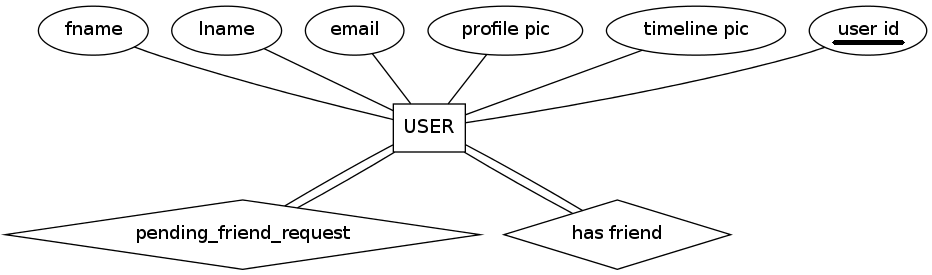
\includegraphics[scale=0.4]{user_friend.png}
\caption{User - User relation}
\label{fig1}
\end{figure}
This relation determines how a user is related to other users in the network. There are two ways:
\begin{itemize}
\item \textbf{pending friend request:} If one user(say,A) sends friend request to other user(say,B), until the user B accepts the request, both users share the \textbf{pending friend request} relation as shown in the \ref{fig1}.
\item \textbf{Friends:} If user B accepts the friend request of user A, then the relationship between them change from pending friends to friends. 
\end{itemize}

\subsection{User - Page relation}
\begin{figure}[h!]
\centering
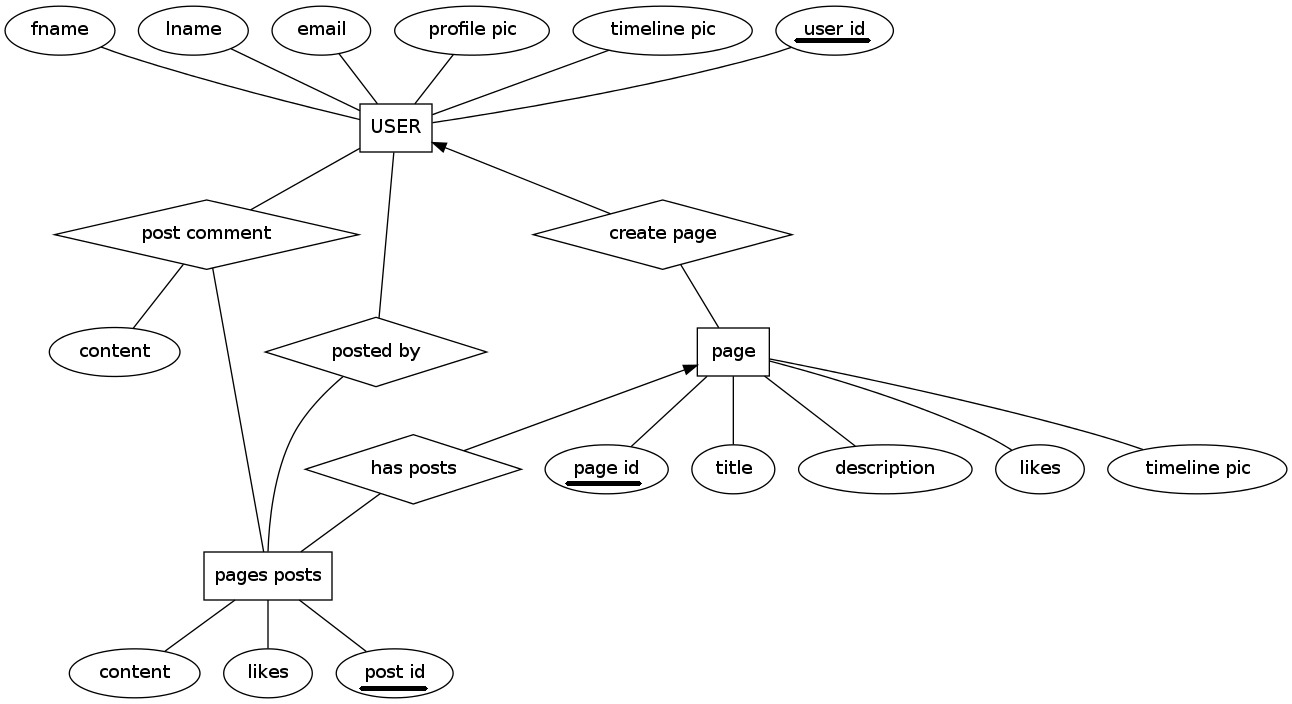
\includegraphics[scale=0.35]{user_pages.png}
\caption{User - Page relation}
\label{fig2}
\end{figure}
Just as each user has a profile, a public page can be created for celebrites, organisations, and other entities. Unlike, user-profile, these pages are public, i.e., they are visible to every user. Users can post and read posts from a page once they like them. Users can be related to a page in following ways:
\begin{itemize}
\item \textbf{Create page:} User can create new pages with attributes like title, description, timeline picture etc.
\item \textbf{Like page:} User can like any number of pages of their interest and start reading and writing posts on the page.
\item \textbf{Page posts:} Each page can have multiple posts by different users and users can even comment on the post by other users.
\end{itemize}

\subsection{User - Group relation}
\begin{figure}[h!]
\centering
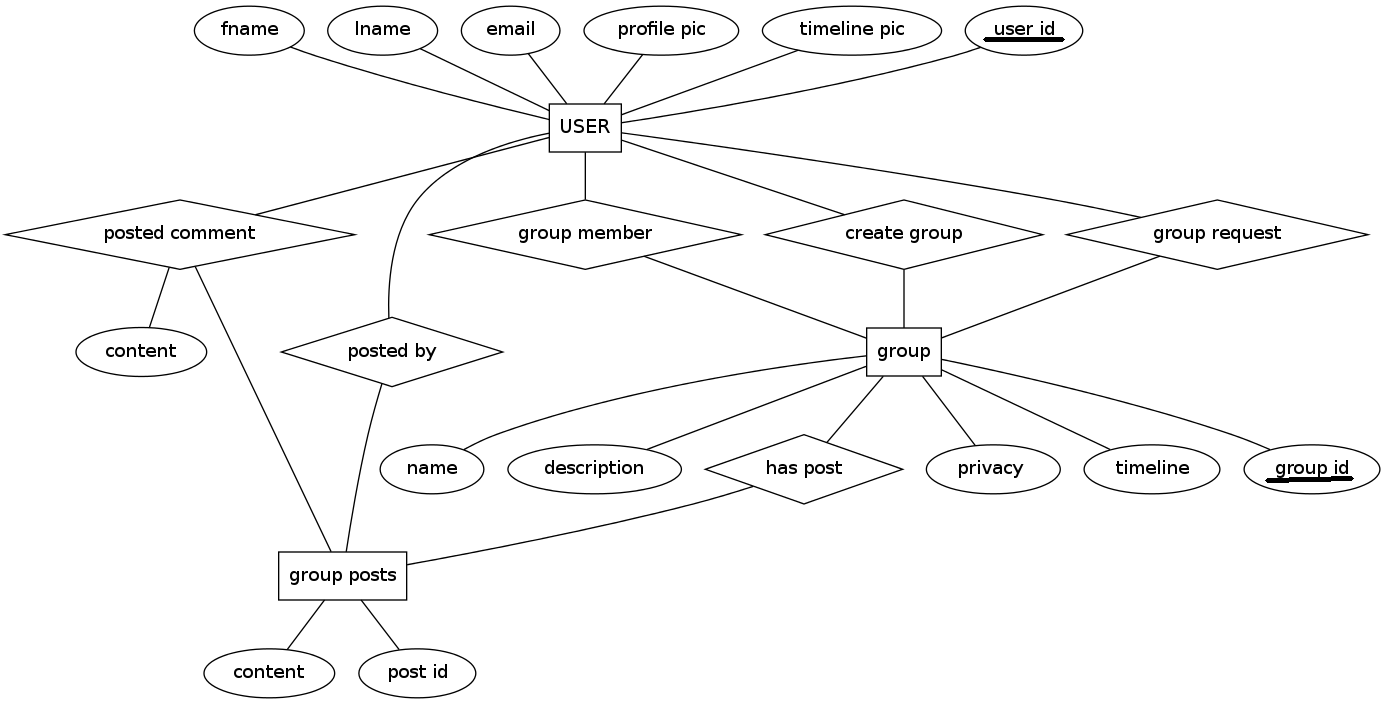
\includegraphics[scale=0.35]{user_groups.png}
\caption{User - Group relation}
\label{fig3}
\end{figure}
Pages are designed to be the profiles for entities, groups are the place for small group communication and for people to share their common interests and express their opinion. When a new group is created by a user, he/she can decide whether to make it publicly available for anyone to join, or require his/her approval for members to join. The relationship between users and groups are described below:
\begin{itemize}
\item \textbf{Create group:} A user can create new groups which can be made public or private as described above. Groups will have attributes like title, description, timeline picture, privacy etc.
\item \textbf{Members:} If a group is public, users can directly become its member. But, if it is private, then a request will be send from the user to the creator of the group. It is upto the creator whether to allow the user to join or not.
\item \textbf{Group posts:} Only members of groups are allowed to view the content and write new posts in the group.
\end{itemize}
\subsection{User - Question relation}
\begin{figure}[h!]
\centering
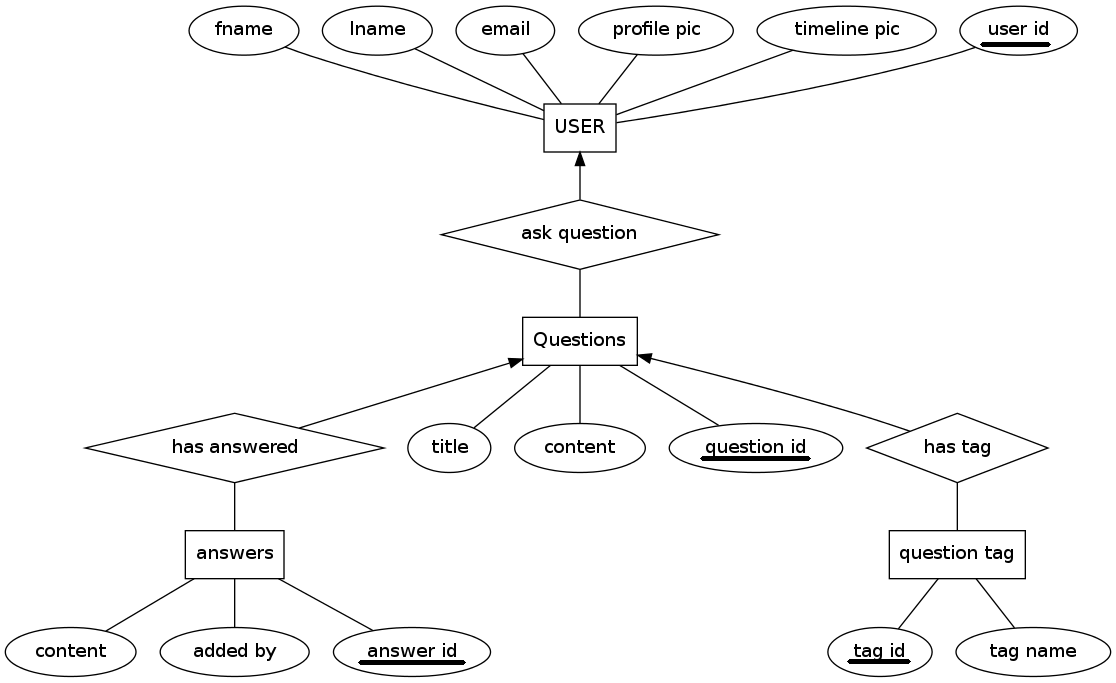
\includegraphics[scale=0.4]{user_question.png}
\caption{User - Question relation}
\label{fig4}
\end{figure}
Apart from pages and groups, a platform is provided to all users to ask question which will be visible to everyone and any user can answer to anyone's query. Users can even search for questions, if already asked by other users and find their answers. User - Question relation can be described as follows:
\begin{itemize}
\item \textbf{Ask questions:} User can ask any question which would be visible to everybody to answer. A question will have attributes - question title, content.
\item \textbf{Has answers:} A question can have multiple answers from multiple users. An answer will contain a content and the user who added that answer.
\item \textbf{Question-tags:} In order to optimize the search query, each question will have certain tags added by user who asked that question. 
\end{itemize} 
\subsection{User - Wall relation}
\begin{figure}[h!]
\centering
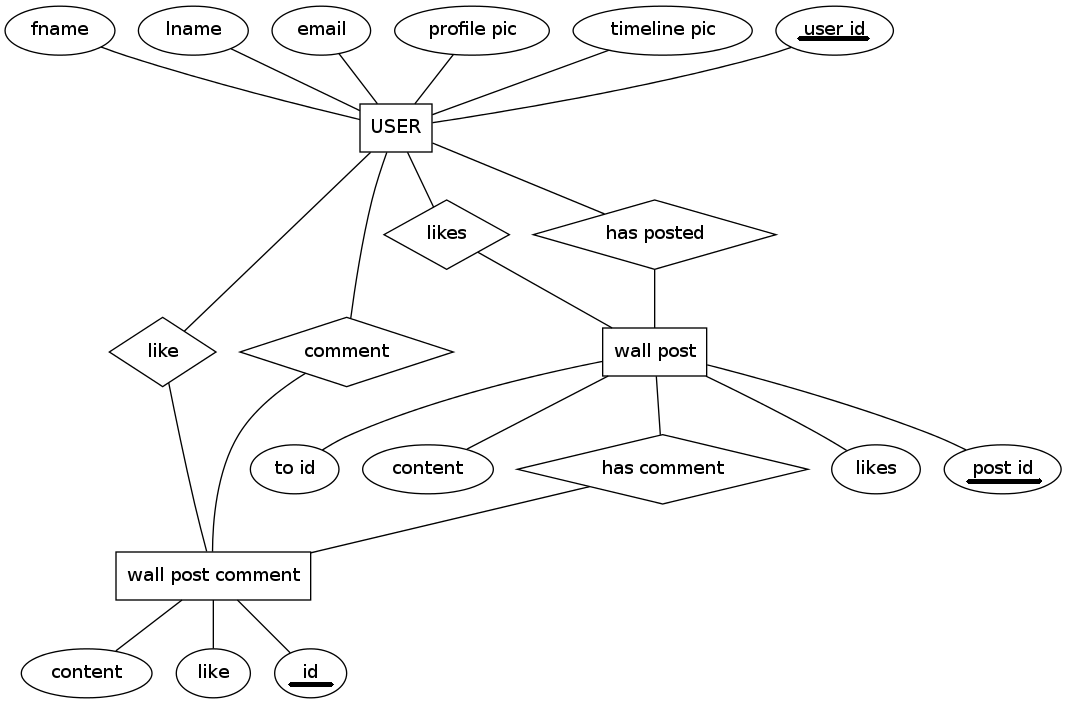
\includegraphics[scale=0.4]{user_wall.png}
\caption{User - Wall relation}
\label{fig5}
\end{figure}
Each user has certain area on his profile, which we call, $wall$, where his/her friends can post or comments. User or his/her friends can like each others post or comments on each other walls. User can interact with walls in following way:
\begin{itemize}
\item \textbf{Wall post:} A user can post to his/her own wall or on the walls of his/her friends. Each post has attributes: content, user on whose wall it is posted, number of likes on the post etc.
\item \textbf{Wall comment:} Users can even comment on the posts by other users which will have same attributes as posts.
\item \textbf{Like post/comment:} A user can like any posts and comments. 
\end{itemize}
\subsection{User - Message relation}
\begin{figure}[h!]
\centering
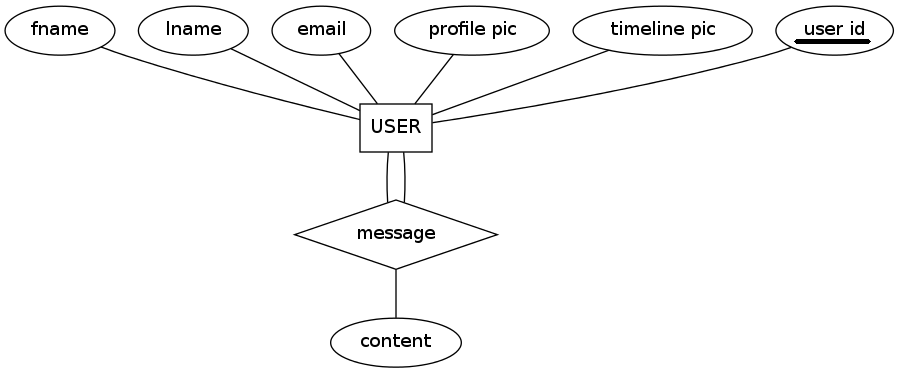
\includegraphics[scale=0.4]{user_messages.png}
\caption{User - Message relation}
\label{fig6}
\end{figure}
Another interesting feature of the social network is the instant messaging. Users can communicate with each other privately using chat and it will store all the previous conversations. Each message will have some content and only two users can be related through messages.

\section{Features}
\subsection{Security measures}
\begin{itemize}
\item \textbf{Email verification:} At the time of registering new users, we need their email address in order to verify their identity. When users sign up , they automatically receive an email request to verify their address. This email is generated using \textbf{sendgrid API}\cite{sendgrid}. To verify, they just need to click on the link in the message. This veriifcation link is generated using 15 hexadecimal of random number which is stored in the database for verification.
\item \textbf{Cookies protection:} Since cookies hold sensitive session information, they need to be verified each time they are used in order to ensure that they have not been tampered. Each time a user login, we store following cookies in the browser:
\begin{itemize}
\item username: Name of the user logged in
\item userid: The id of the user, which acts as primary key.
\item checksum: A 15 hexadecimal long random number
\end{itemize}
userid and checksum is also stored in the database on server side and everytime cookies are used, checksum stored in the browser is matched with that stored in the database. If matching fails, user is logged out immediately and need to login again, otherwise, required action is executed. This ensures integrality of cookies. 
\item \textbf{Groups privacy:} Since, groups can be private, a non-member is not allowed to view the content of the group unless his request to join group is accepted by the creator of the group.
\item \textbf{Password change:} We have also given the feature of changing password in case the password of any user is compromised or user forgets his/her password. The password is sent via email, which can be later changed by user.
\end{itemize}
\subsection{Additional features:}
\begin{itemize}
\item \textbf{Search engine:} We have developed a very user friendly search engine. The search engine keeps on matching the incomplete query filled by user and return all the related responses from the database in the real time using \textbf{auto-complete javascript library}\cite{autocomplete}. Search query can be categorised as follows:
\begin{itemize}
\item Search people: User can simply type the name of the person and all related results can be seen in the drop-down.
\item Search page: User can search for a page through its title using search query - \textbf{page : $<title>$}
\item Search group: User can search for a group through group-name using search query - \textbf{group : $<name>$}
\item Search question: User can search for any question asked by some user through its tag or title using search query - \textbf{question : $<title/tags>$}.
\end{itemize}
In all cases, query is matched from database and top five results are displayed to the user.

\item \textbf{Advanced search:} Apart from directly searching for people, pages and groups, we have implemented advanced query search which allows user to refine their search using specific queries. Following type of advanced queries are supported by us:
\begin{itemize}
\item friends who live in $<city>$
\item people who live in $<city>$ 
\item friends who study in $<university>$
\item people who study in $<university>$
\item friends who like $<page>$ 
\item people who like $<page>$
\end{itemize}
\end{itemize}
\section{Future work}
\begin{itemize}
\item The user-interface can be improved.
\item We can use ajax more extensively so that we have to refresh pages less often. 
\item We can implement graph database to improve the model of our database.
\end{itemize}
\begin{thebibliography}{99} 
 \bibitem{paperclip} https\://github.com/thoughtbot/paperclip
 \bibitem{join} http\://guides.rubyonrails.org/association\_basics.html 
 \bibitem{autocomplete} http\://api.jqueryui.com/autocomplete/ 
 \bibitem{rubyonrails} http\://ruby.railstutorial.org/ruby-on-rails-tutorial-book
 \bibitem{sendgrid}http\://sendgrid.com/docs/Code\_Examples/ruby.html
 \bibitem{bootstrap}http\://getbootstrap.com/css/
 \end{thebibliography}
\end{document}